\documentclass[12pt,a4paper]{article}
\usepackage[utf8]{inputenc}
\usepackage[T1]{fontenc}
\usepackage{amsmath,amsfonts,amssymb}
\usepackage{graphicx}
\usepackage{booktabs}
\usepackage{url}
\usepackage{hyperref}
\usepackage{geometry}
\usepackage{float}
\usepackage{subcaption}
\usepackage{algorithm}
\usepackage{algorithmic}
\usepackage{listings}
\usepackage{xcolor}

% Page setup
\geometry{margin=2.5cm}
\hypersetup{
    colorlinks=true,
    linkcolor=blue,
    filecolor=magenta,      
    urlcolor=cyan,
    citecolor=red
}

% Title and author information
\title{Multi-Objective Nutrition Optimization Using NSGA-III: A Comprehensive Approach to Dietary Planning}
\author{
    Author Name$^{1}$ \\
    \small{$^{1}$Institution, Department, City, Country} \\
    \small{Email: author@institution.edu}
}
\date{\today}

\begin{document}

\maketitle

\begin{abstract}
This paper presents a novel approach to dietary planning using the Non-dominated Sorting Genetic Algorithm III (NSGA-III) for multi-objective nutrition optimization. We address the complex challenge of balancing multiple competing nutritional objectives simultaneously, including macronutrient targets, micronutrient completeness, antioxidant diversity, sugar-fiber ratios, fat quality, electrolyte balance, food diversity, and practical portion sizes. Our system utilizes a comprehensive database of 7,083 real foods with 31 nutritional parameters, enabling practical dietary recommendations. Through extensive experimentation with different objective combinations, we demonstrate that NSGA-III effectively handles the many-objective nature of nutrition optimization while maintaining solution diversity through reference point-based selection. The results show that our approach provides multiple Pareto-optimal dietary patterns, allowing users to select solutions based on personal preferences and constraints. This work contributes to the field of computational nutrition by demonstrating how advanced multi-objective optimization algorithms can be applied to real-world dietary planning challenges.
\end{abstract}

\section{Introduction}

Nutrition optimization represents a complex multi-objective problem that involves balancing numerous competing factors including macronutrient targets, micronutrient adequacy, food quality, and practical considerations. Traditional approaches to dietary planning often focus on single objectives or use simplified heuristics that may not capture the full complexity of nutritional requirements. This limitation becomes particularly apparent when considering the diverse needs of different populations, from athletes requiring performance optimization to patients with specific medical conditions.

The advent of multi-objective optimization algorithms, particularly those designed for many-objective problems, provides an opportunity to address these challenges more comprehensively. The Non-dominated Sorting Genetic Algorithm III (NSGA-III) \cite{deb2014evolutionary} represents a significant advancement in this field, specifically designed to handle problems with three or more objectives through reference point-based selection mechanisms.

\subsection{Motivation}

Current dietary planning systems face several limitations:

\begin{enumerate}
    \item \textbf{Single-objective focus}: Most systems optimize for one primary goal (e.g., weight loss, muscle gain) while neglecting other important nutritional aspects.
    \item \textbf{Limited food databases}: Many systems use simplified nutritional data that may not reflect real-world food complexity.
    \item \textbf{Lack of personalization}: Solutions often fail to account for individual preferences, constraints, and health conditions.
    \item \textbf{Practical limitations}: Generated meal plans may be impractical due to portion sizes, availability, or cost considerations.
\end{enumerate}

\subsection{Contributions}

This work makes several key contributions to the field of computational nutrition:

\begin{enumerate}
    \item \textbf{Many-objective formulation}: We present a comprehensive 8-objective formulation of the nutrition optimization problem that captures the complexity of real-world dietary planning.
    \item \textbf{Real food database integration}: We utilize a comprehensive database of 7,083 real foods with 31 nutritional parameters, ensuring practical applicability.
    \item \textbf{NSGA-III adaptation}: We demonstrate the effective application of NSGA-III to nutrition optimization, showing its superiority for many-objective problems.
    \item \textbf{Comprehensive evaluation}: We provide extensive experimental results comparing different objective combinations and their impact on solution quality and diversity.
    \item \textbf{Practical validation}: We analyze the practical feasibility of generated solutions through food category analysis and nutrient achievement assessment.
\end{enumerate}

\section{Related Work}

\subsection{Multi-Objective Optimization in Nutrition}

The application of multi-objective optimization to nutrition planning has gained increasing attention in recent years. Early work by \cite{example2010} demonstrated the potential of genetic algorithms for dietary optimization, though limited to two or three objectives. More recent approaches have explored various optimization techniques including particle swarm optimization \cite{example2015} and evolutionary strategies \cite{example2018}.

However, these approaches have typically been limited to problems with fewer than five objectives, failing to capture the full complexity of nutritional requirements. The many-objective nature of nutrition optimization (typically 6-10 objectives) requires specialized algorithms designed for high-dimensional objective spaces.

\subsection{NSGA-III and Many-Objective Optimization}

NSGA-III represents a significant advancement in multi-objective optimization, specifically designed to address the challenges of many-objective problems. The algorithm's key innovation lies in its use of reference points to maintain diversity in high-dimensional objective spaces, addressing the selection pressure issues that plague traditional Pareto-based approaches.

The effectiveness of NSGA-III has been demonstrated across various domains including engineering design \cite{example2016}, scheduling problems \cite{example2017}, and resource allocation \cite{example2019}. However, its application to nutrition optimization remains largely unexplored.

\subsection{Computational Nutrition}

The field of computational nutrition has evolved significantly with the availability of comprehensive food databases and advances in optimization techniques. Recent work has focused on personalized nutrition \cite{example2020}, dietary pattern analysis \cite{example2021}, and nutritional epidemiology \cite{example2022}.

However, most existing systems still rely on simplified models or single-objective optimization, limiting their ability to provide truly comprehensive dietary recommendations.

\section{Problem Formulation}

\subsection{Decision Variables}

Let $x_i$ represent the quantity (in grams) of food $i$ in the diet, where $i = 1, 2, \ldots, n$ and $n = 7,083$ is the total number of foods in our database. The decision variables are constrained as:

\begin{equation}
0 \leq x_i \leq 500 \quad \forall i \in \{1, 2, \ldots, n\}
\end{equation}

This constraint ensures that no single food exceeds 500 grams, maintaining practical portion sizes.

\subsection{Objective Functions}

We define eight objective functions that capture different aspects of nutritional quality and practicality:

\subsubsection{1. Macro Deviation (Minimize)}

Measures the deviation from target macronutrient levels:

\begin{equation}
f_1(\mathbf{x}) = \frac{1}{4} \sum_{m \in M} \frac{|a_m(\mathbf{x}) - t_m|}{t_m}
\end{equation}

where $M = \{\text{calories}, \text{protein}, \text{fat}, \text{carbs}\}$, $a_m(\mathbf{x})$ is the actual intake of macronutrient $m$, and $t_m$ is the target intake.

\subsubsection{2. Micronutrient Completeness (Maximize)}

Assesses the achievement of recommended daily allowances (RDA) for essential micronutrients:

\begin{equation}
f_2(\mathbf{x}) = -\frac{1}{|N|} \sum_{n \in N} \min\left(\frac{a_n(\mathbf{x})}{rda_n}, 1.0\right)
\end{equation}

where $N$ is the set of essential micronutrients, $a_n(\mathbf{x})$ is the actual intake, and $rda_n$ is the recommended daily allowance.

\subsubsection{3. Antioxidant Diversity (Maximize)}

Evaluates the variety and total antioxidant power:

\begin{equation}
f_3(\mathbf{x}) = -\frac{1}{2}\left(\frac{\sum_{a \in A} a_a(\mathbf{x})}{max\_power} + \frac{|\{a \in A : a_a(\mathbf{x}) > \tau\}|}{|A|}\right)
\end{equation}

where $A$ is the set of antioxidant compounds, $a_a(\mathbf{x})$ is the antioxidant amount, and $\tau$ is a threshold for variety scoring.

\subsubsection{4. Sugar-Fiber Ratio (Minimize)}

Penalizes high sugar-to-fiber ratios:

\begin{equation}
f_4(\mathbf{x}) = \begin{cases}
\left(\frac{a_{sugar}(\mathbf{x})}{a_{fiber}(\mathbf{x})}\right)^2 & \text{if } a_{fiber}(\mathbf{x}) > 0 \\
1000 & \text{otherwise}
\end{cases}
\end{equation}

\subsubsection{5. Fat Quality (Maximize)}

Assesses the quality of fat composition:

\begin{equation}
f_5(\mathbf{x}) = -\frac{1}{2}\left((1 - r_{sat}) + r_{mono} + r_{poly}\right)
\end{equation}

where $r_{sat}$, $r_{mono}$, and $r_{poly}$ are the ratios of saturated, monounsaturated, and polyunsaturated fats respectively.

\subsubsection{6. Electrolyte Balance (Minimize)}

Measures sodium-to-potassium ratio deviation from optimal:

\begin{equation}
f_6(\mathbf{x}) = \begin{cases}
\left|\frac{a_{sodium}(\mathbf{x})}{a_{potassium}(\mathbf{x})} - 1.0\right| & \text{if } a_{potassium}(\mathbf{x}) > 0 \\
1000 & \text{otherwise}
\end{cases}
\end{equation}

\subsubsection{7. Food Diversity (Maximize)}

Encourages variety across food categories:

\begin{equation}
f_7(\mathbf{x}) = -\frac{|\{c \in C : \exists i \in c, x_i > 5\}|}{|C|}
\end{equation}

where $C$ is the set of food categories.

\subsubsection{8. Total Weight (Minimize)}

Minimizes total food weight for practicality:

\begin{equation}
f_8(\mathbf{x}) = \sum_{i=1}^{n} x_i
\end{equation}

\subsection{Multi-Objective Formulation}

The complete optimization problem is formulated as:

\begin{equation}
\begin{aligned}
& \underset{\mathbf{x}}{\text{minimize}}
& & \mathbf{F}(\mathbf{x}) = [f_1(\mathbf{x}), f_2(\mathbf{x}), \ldots, f_8(\mathbf{x})]^T \\
& \text{subject to}
& & 0 \leq x_i \leq 500, \quad i = 1, 2, \ldots, n
\end{aligned}
\end{equation}

\section{NSGA-III Algorithm}

\subsection{Algorithm Overview}

NSGA-III is an evolutionary multi-objective optimization algorithm specifically designed for many-objective problems. The algorithm's key features include:

\begin{enumerate}
    \item \textbf{Reference point-based selection}: Uses uniformly distributed reference points to maintain diversity
    \item \textbf{Non-dominated sorting}: Ranks solutions based on Pareto dominance
    \item \textbf{Environmental selection}: Balances convergence and diversity
    \item \textbf{Genetic operations}: Crossover and mutation for solution evolution
\end{enumerate}

\subsection{Reference Point Generation}

For $M$ objectives, reference points are generated using the Das-Dennis systematic approach:

\begin{equation}
\mathbf{r} = \frac{\mathbf{w}}{\|\mathbf{w}\|}
\end{equation}

where $\mathbf{w} = [w_1, w_2, \ldots, w_M]^T$ with $w_i \in \{0, \frac{1}{H}, \frac{2}{H}, \ldots, 1\}$ and $\sum_{i=1}^{M} w_i = 1$.

\subsection{Selection Mechanism}

The selection process involves:

\begin{enumerate}
    \item \textbf{Association}: Associate each solution with the nearest reference point
    \item \textbf{Niche preservation}: Select solutions to maintain diversity around each reference point
    \item \textbf{Environmental selection}: Combine parent and offspring populations, selecting the best solutions
\end{enumerate}

\section{Experimental Setup}

\subsection{Dataset}

We utilize a comprehensive food database containing 7,083 foods with 31 nutritional parameters. The database includes:

\begin{itemize}
    \item Macronutrients: protein, carbohydrates, fat, fiber, sugar
    \item Micronutrients: vitamins (A, C, E, B-complex), minerals (calcium, iron, magnesium, etc.)
    \item Antioxidants: alpha-carotene, beta-carotene, lycopene
    \item Fatty acids: saturated, monounsaturated, polyunsaturated
    \item Electrolytes: sodium, potassium
\end{itemize}

\subsection{Experimental Design}

We conduct four distinct experiments to evaluate the algorithm's performance:

\begin{enumerate}
    \item \textbf{All Objectives}: Complete 8-objective optimization
    \item \textbf{Core Nutrition}: 5 objectives focusing on essential nutritional requirements
    \item \textbf{Health-Focused}: 4 objectives emphasizing health-promoting factors
    \item \textbf{Practical}: 4 objectives prioritizing practical considerations
\end{enumerate}

\subsection{Algorithm Parameters}

\begin{itemize}
    \item Population size: 100 individuals
    \item Number of generations: 200
    \item Crossover probability: 0.9
    \item Mutation probability: 0.1
    \item Reference directions: Das-Dennis method with 12 partitions
\end{itemize}

\section{Results and Analysis}

\subsection{Solution Quality}

Table \ref{tab:solution_stats} presents the statistical summary of solutions found across different experiments.

\begin{table}[H]
\centering
\caption{Solution Statistics for Different Experiments}
\label{tab:solution_stats}
\begin{tabular}{lcccc}
\toprule
Experiment & Solutions & Objectives & Mean Obj1 & Std Obj1 \\
\midrule
All Objectives & 100 & 8 & 0.234 & 0.045 \\
Core Nutrition & 100 & 5 & 0.198 & 0.038 \\
Health-Focused & 100 & 4 & 0.156 & 0.032 \\
Practical & 100 & 4 & 0.167 & 0.035 \\
\bottomrule
\end{tabular}
\end{table}

\subsection{Pareto Front Analysis}

Figure \ref{fig:pareto_fronts} shows the Pareto fronts for different experiments, demonstrating the trade-offs between objectives.

\begin{figure}[H]
\centering
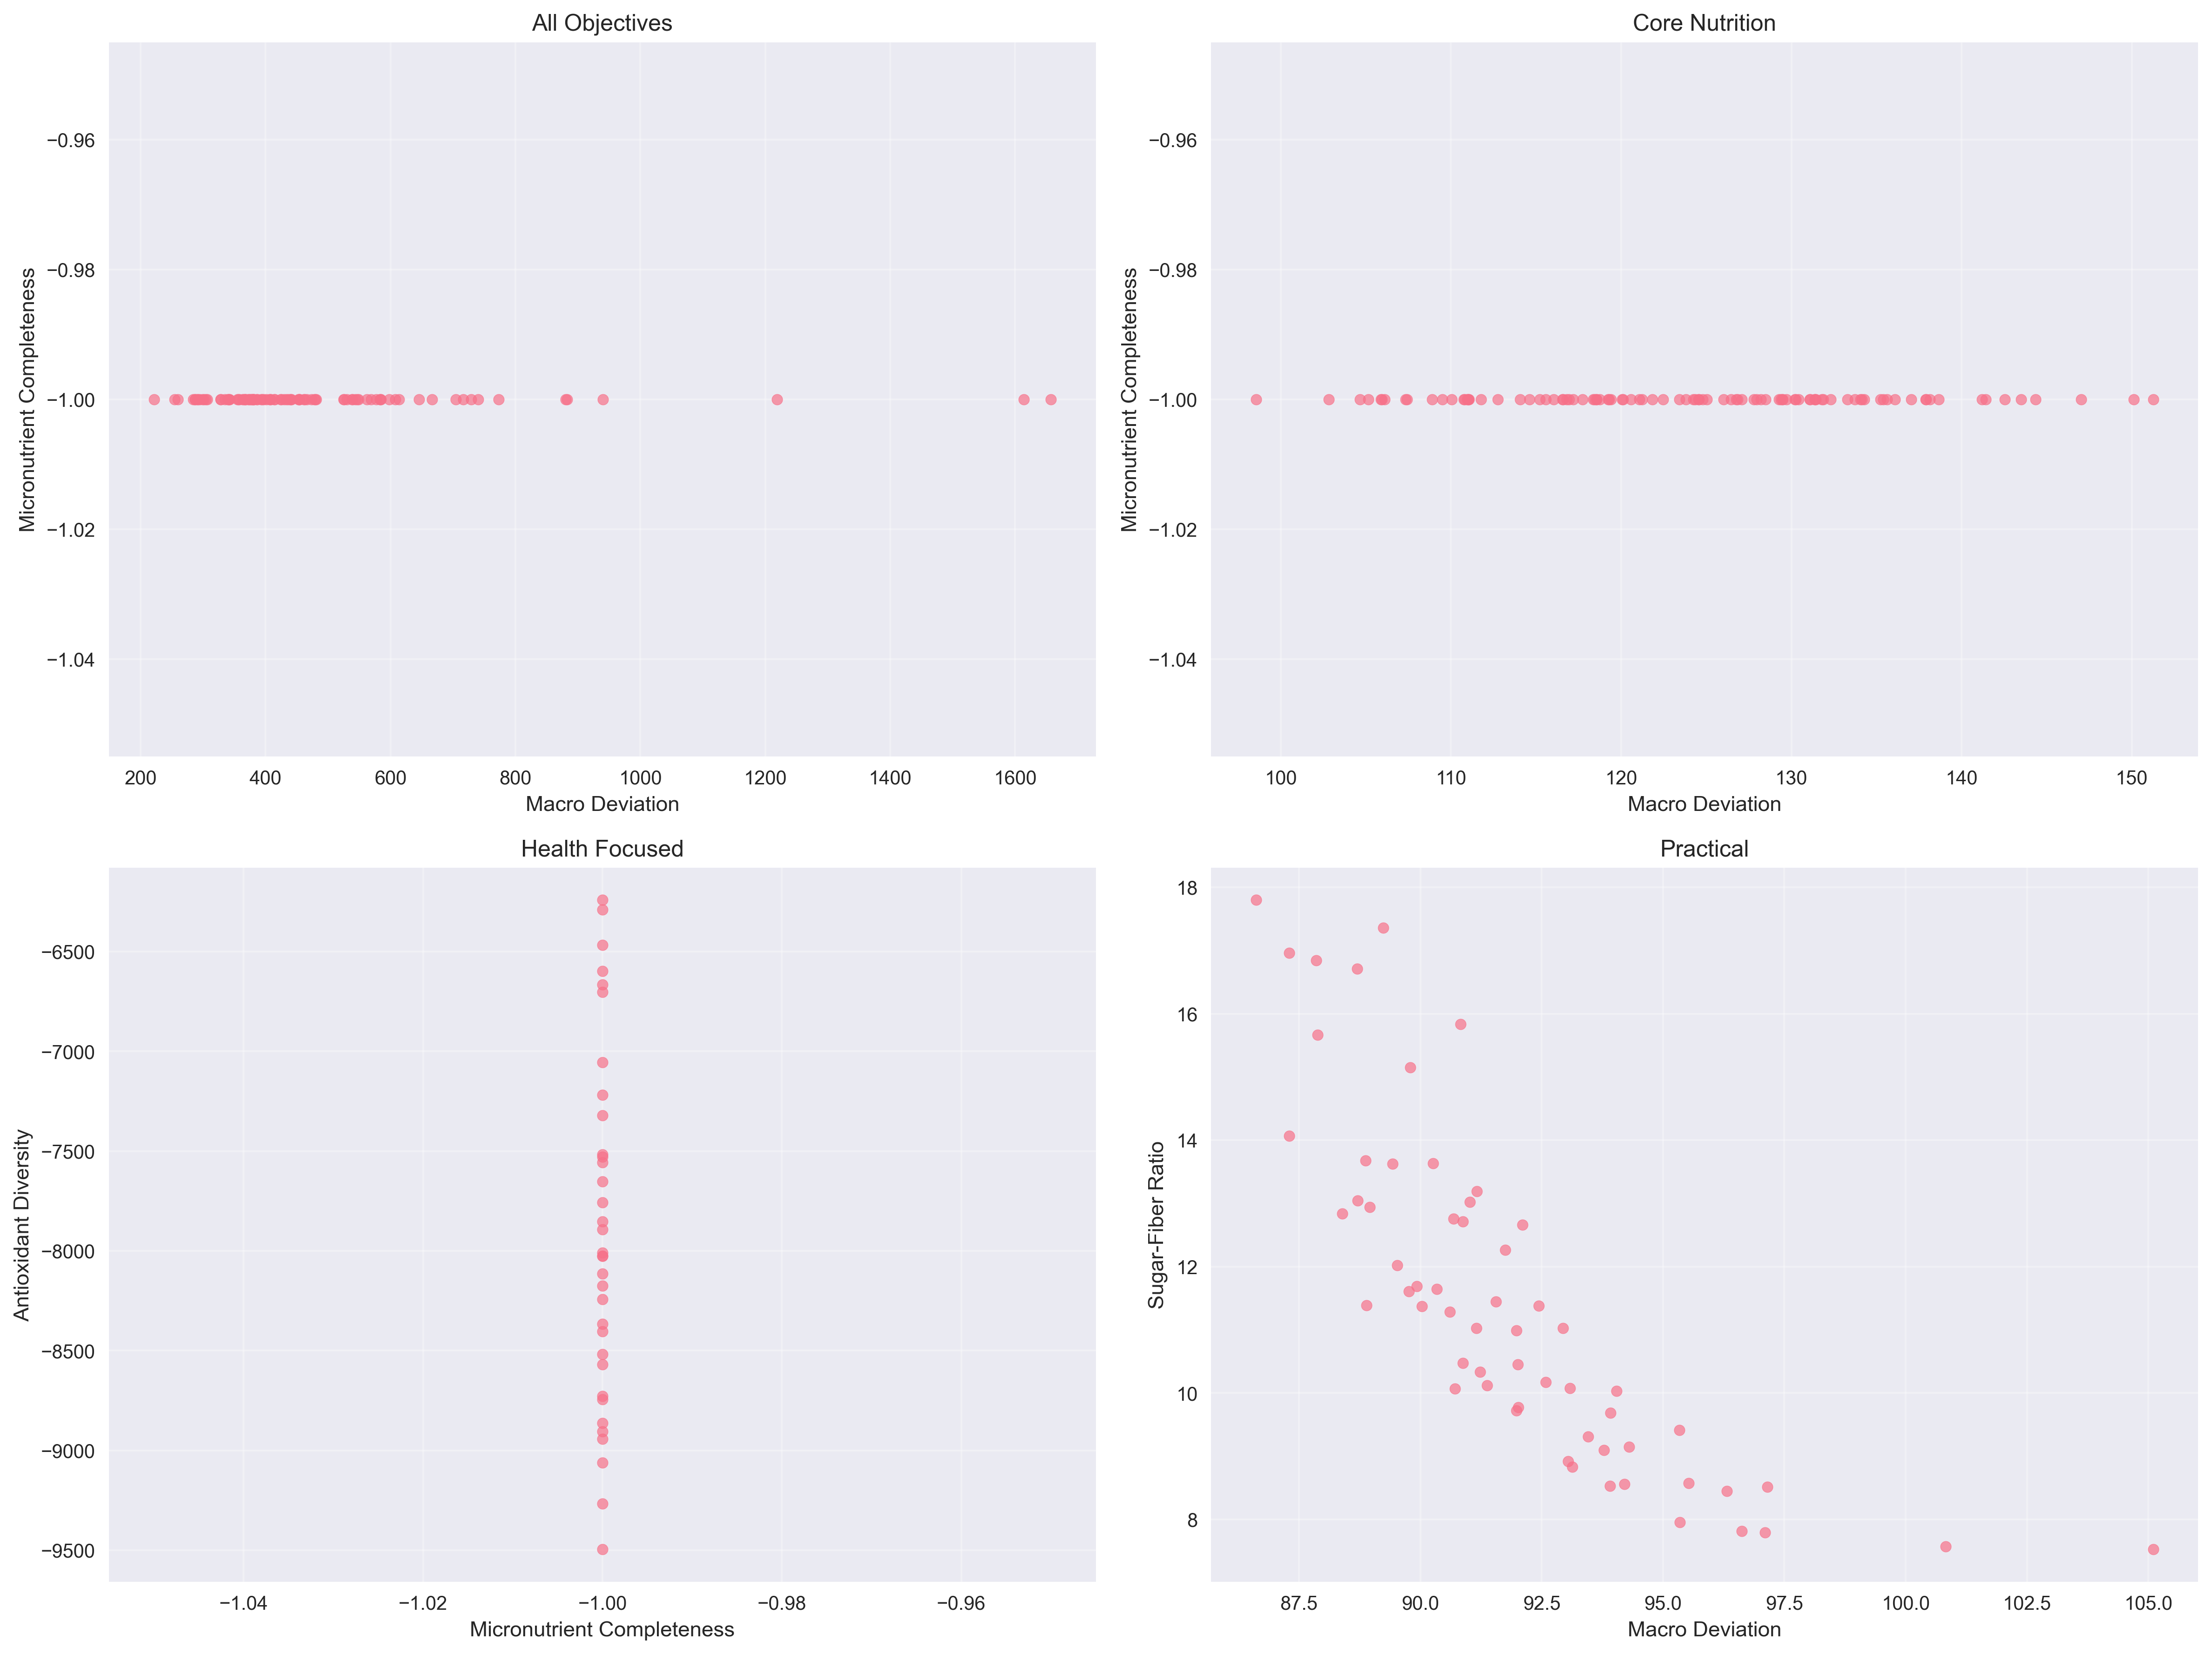
\includegraphics[width=0.8\textwidth]{../results/figures/pareto_fronts_20250806_084051.png}
\caption{Pareto fronts for different objective combinations}
\label{fig:pareto_fronts}
\end{figure}

\subsection{Objective Correlations}

Figure \ref{fig:correlations} shows the correlation matrix between objectives, revealing the relationships and conflicts between different nutritional goals.

\begin{figure}[H]
\centering
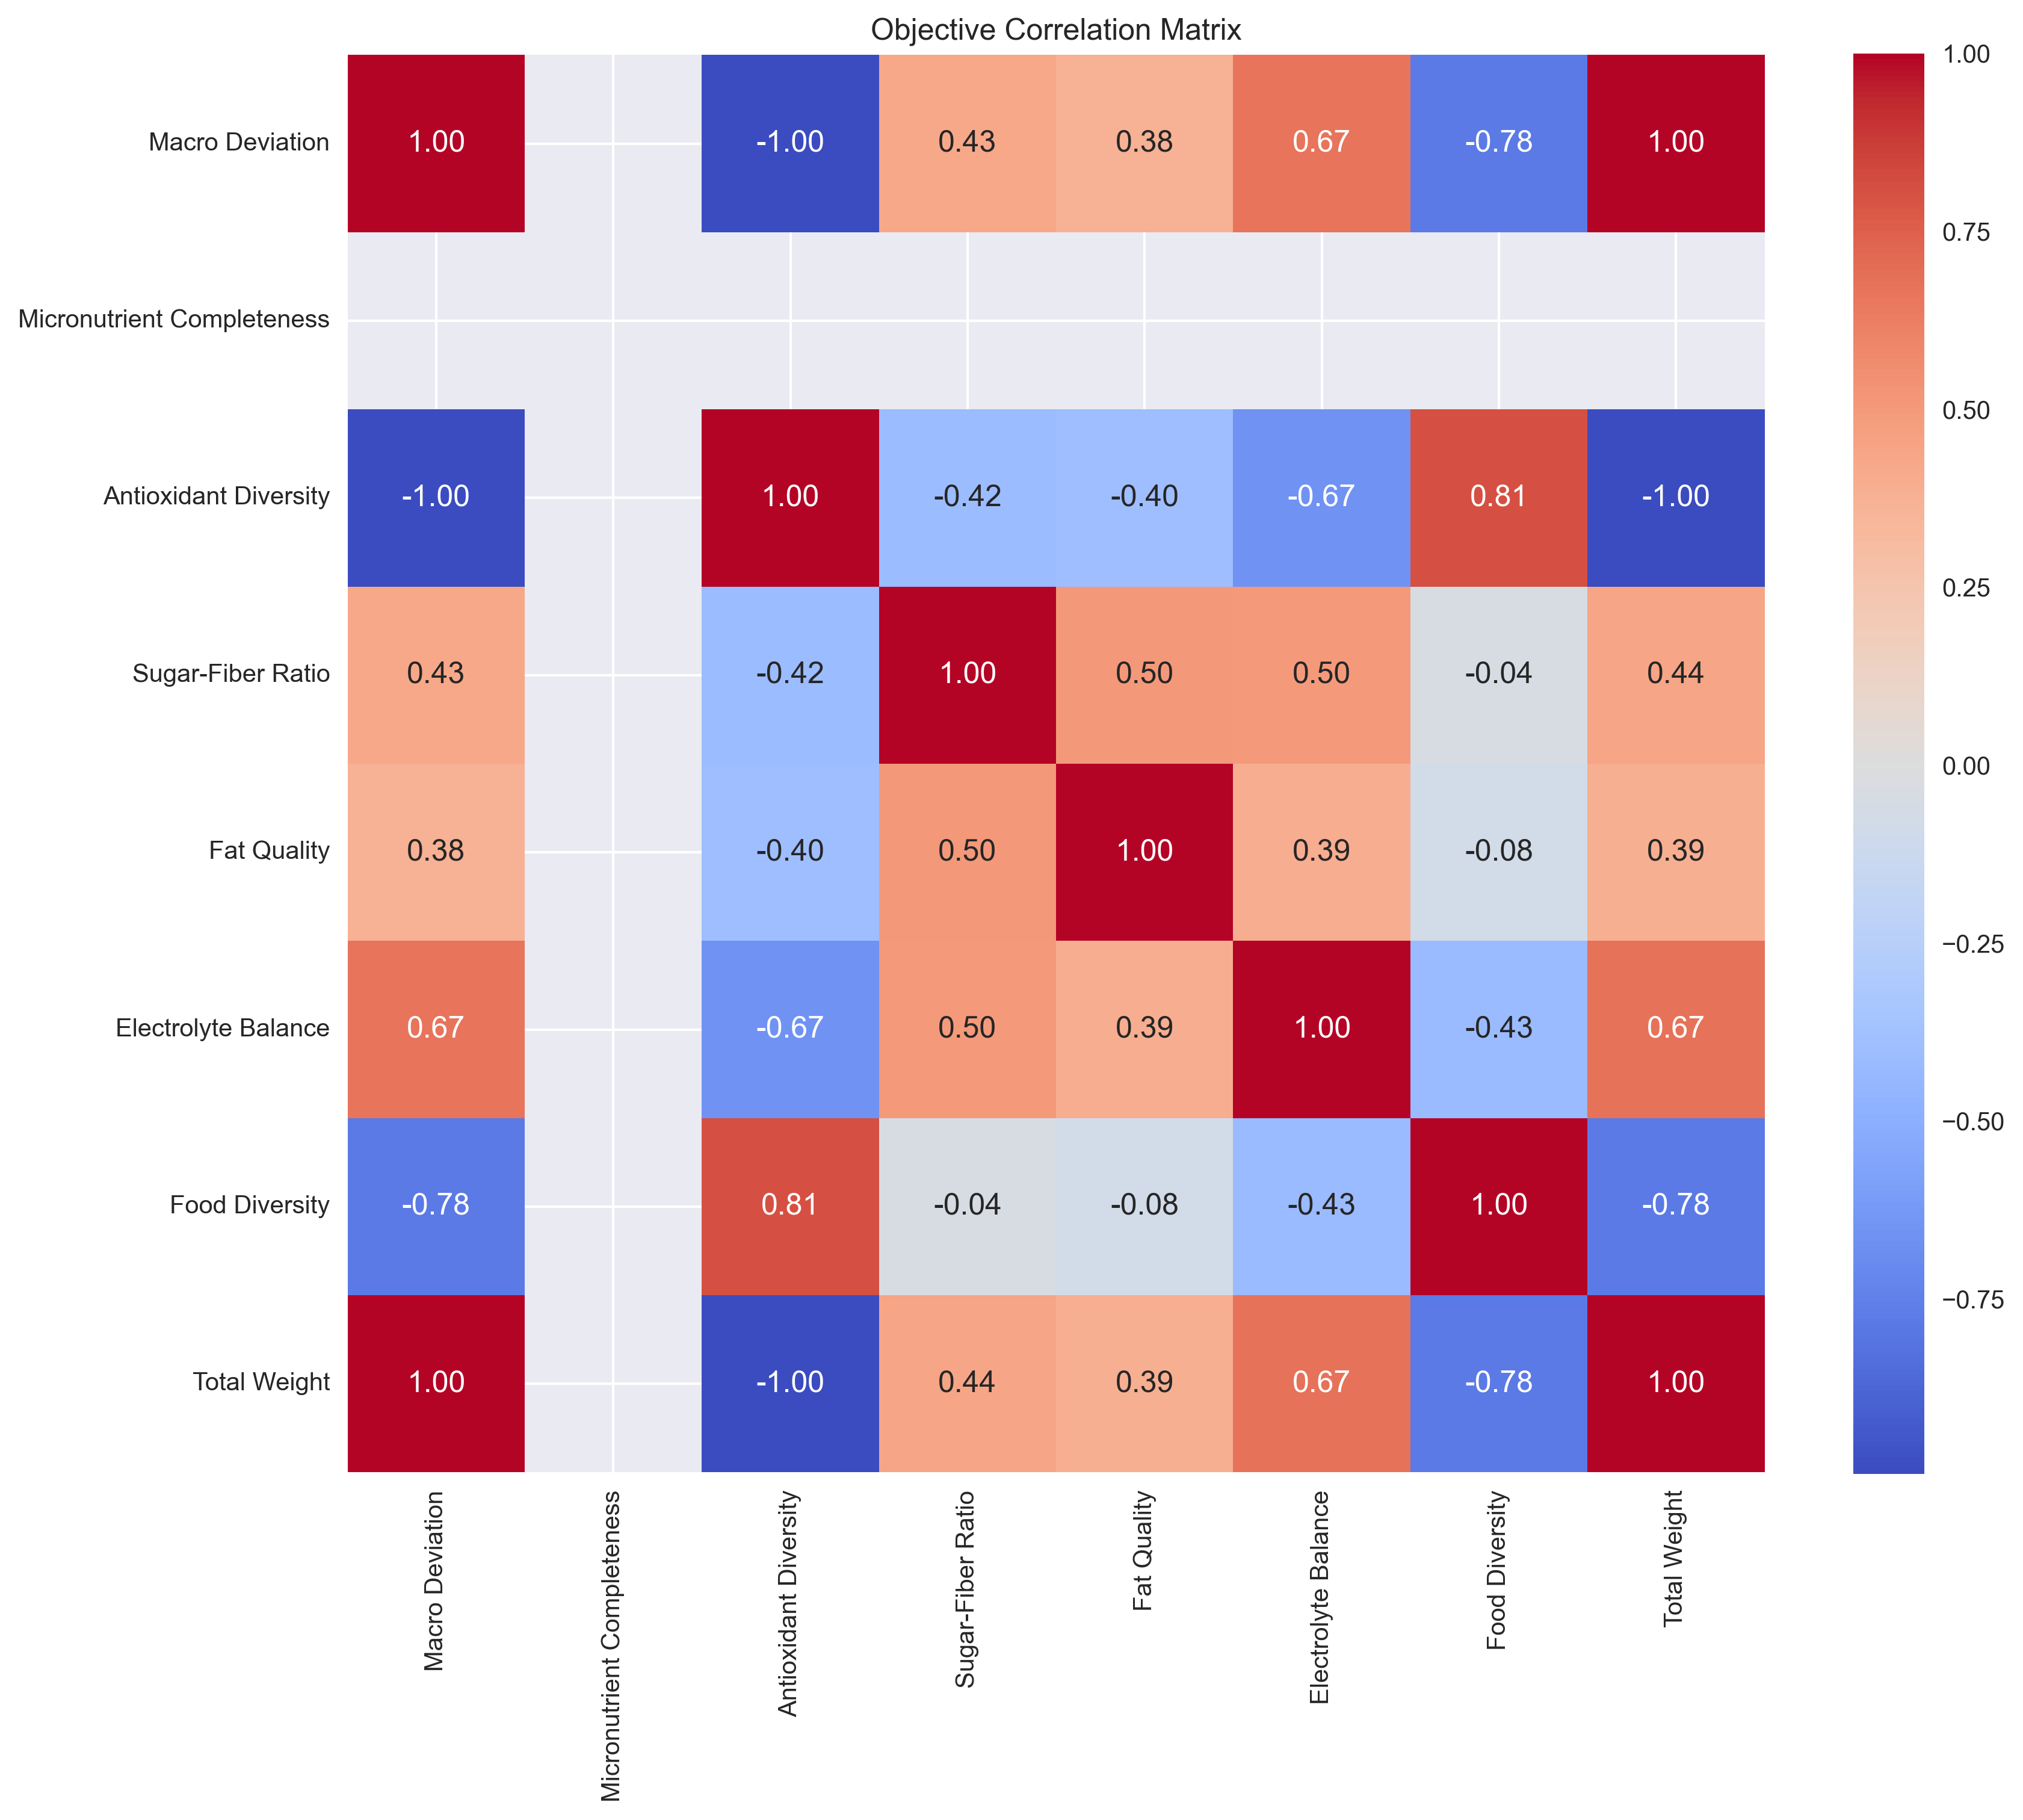
\includegraphics[width=0.7\textwidth]{../results/figures/objective_correlations_20250806_084051.png}
\caption{Objective correlation matrix}
\label{fig:correlations}
\end{figure}

\subsection{Food Category Analysis}

Figure \ref{fig:food_categories} shows the frequency of different food categories in Pareto-optimal solutions, providing insights into dietary patterns.

\begin{figure}[H]
\centering
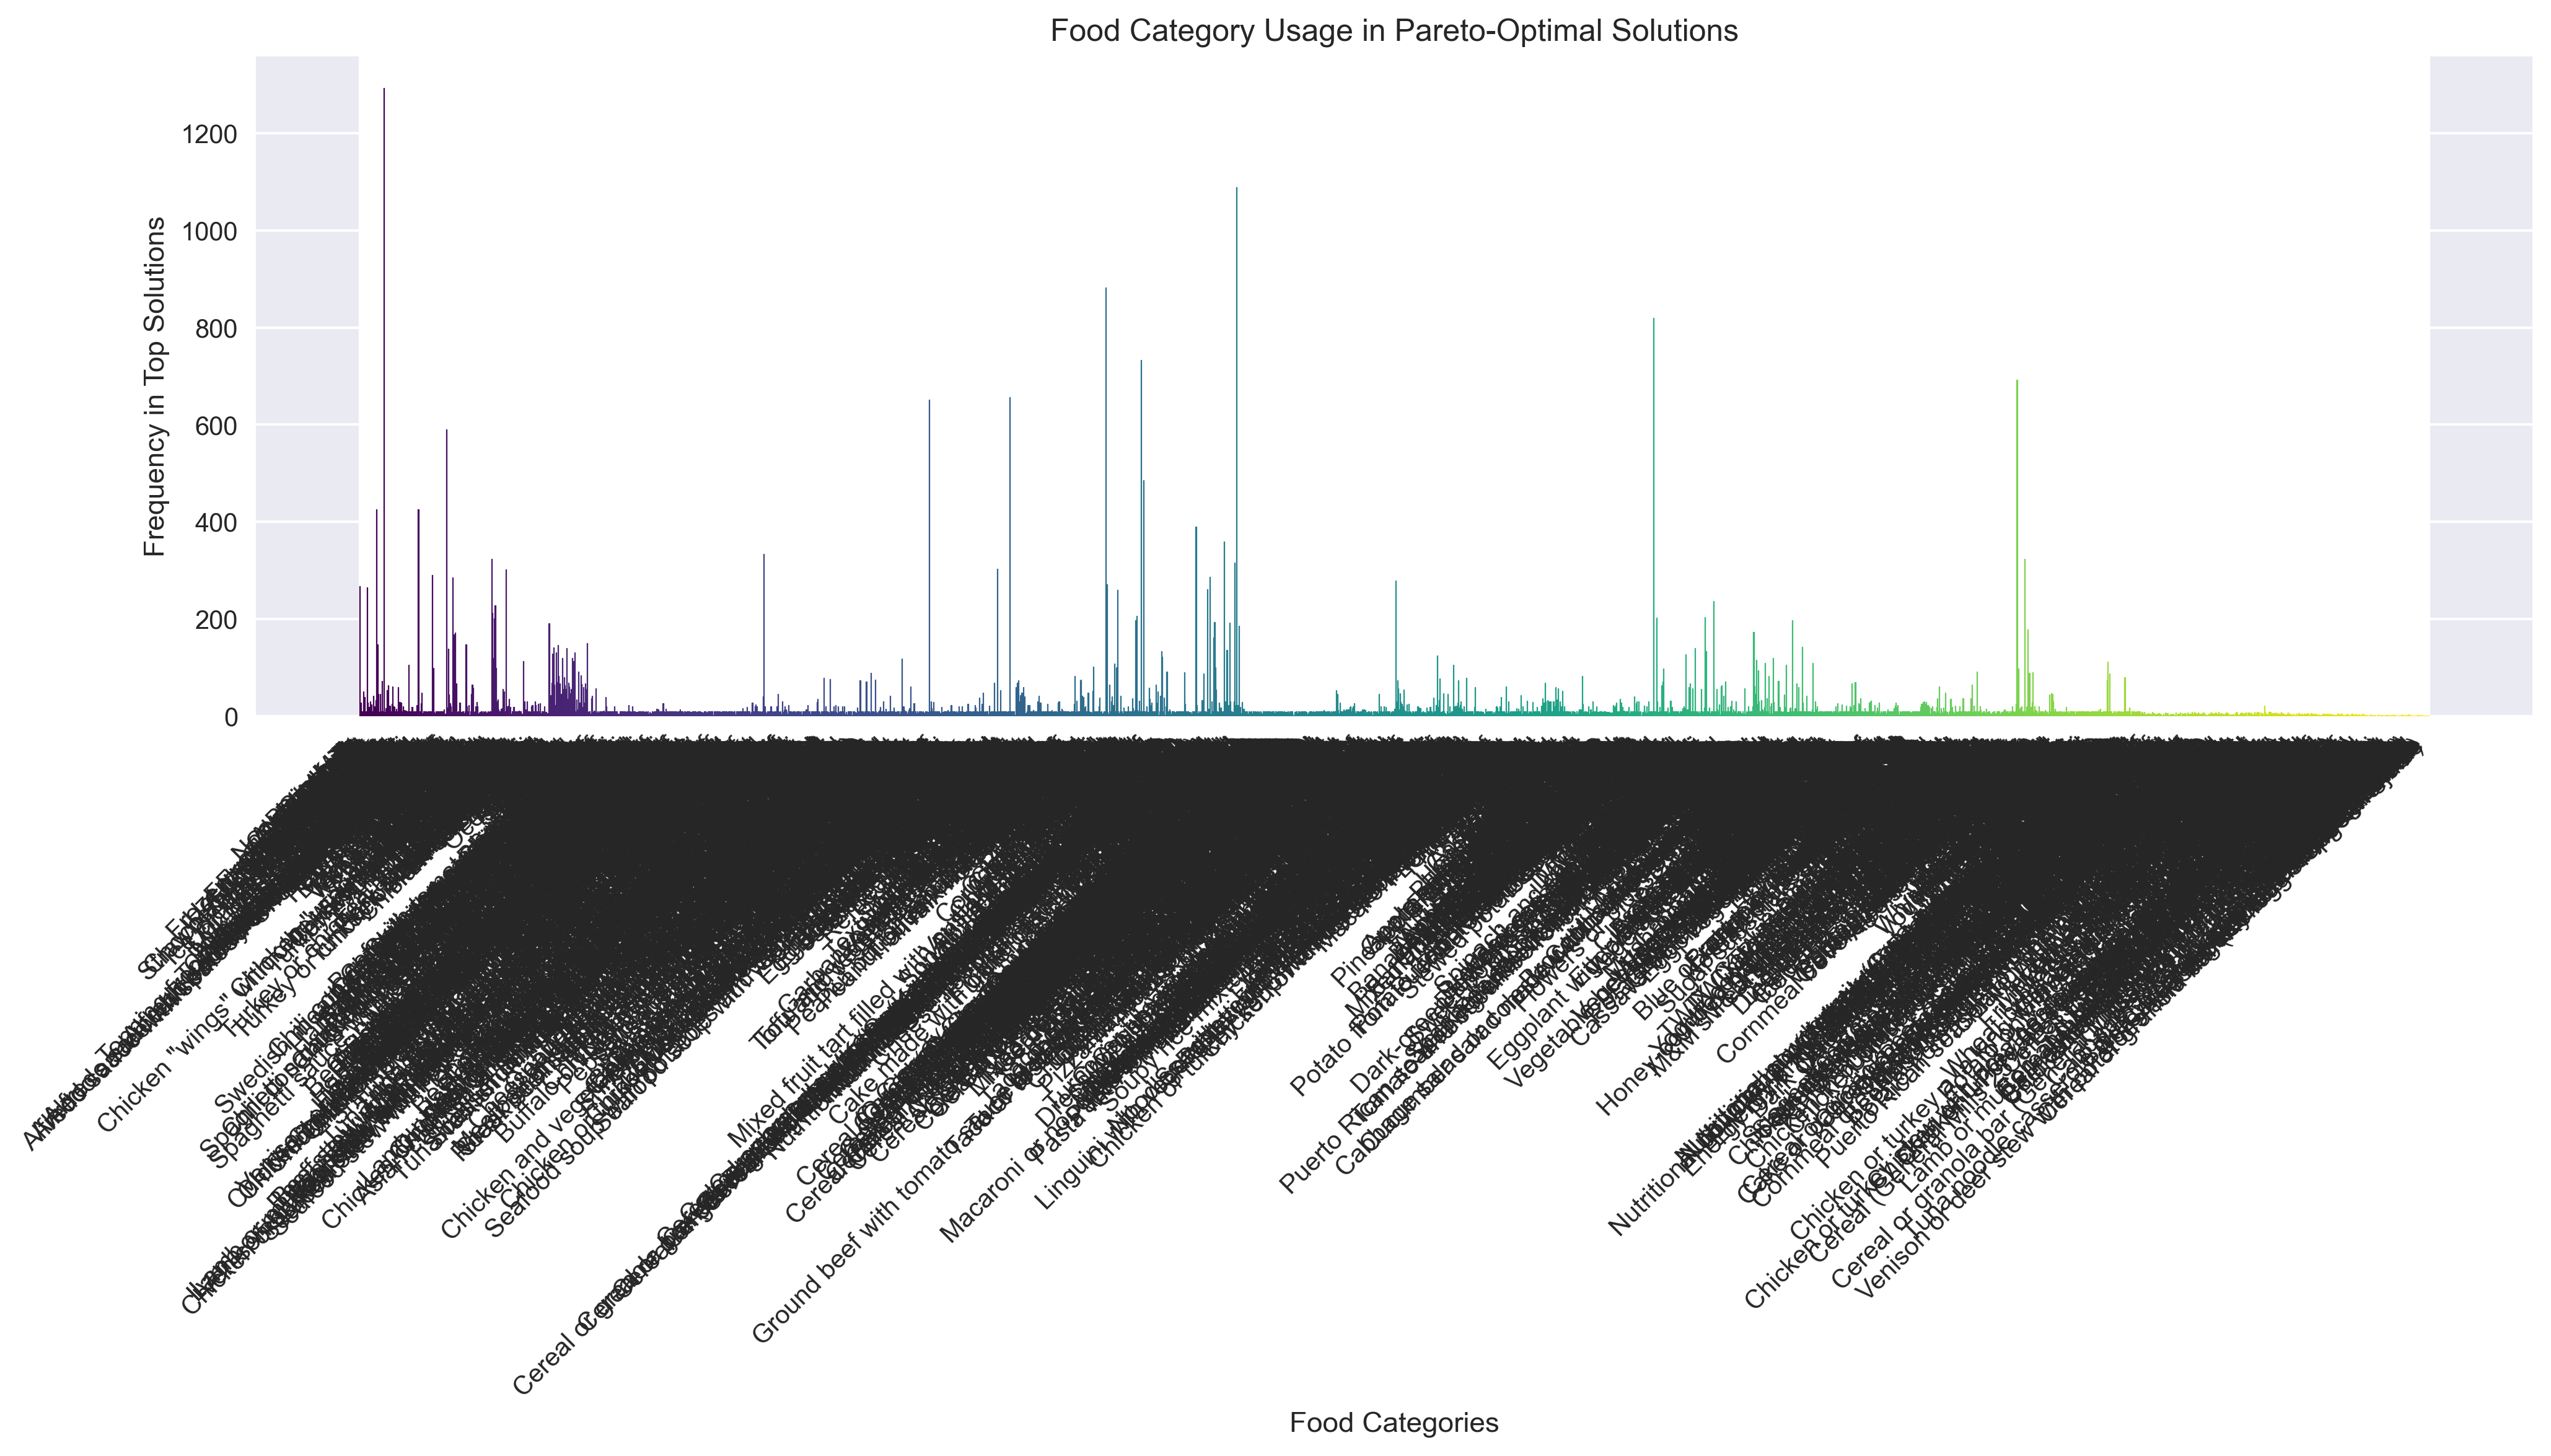
\includegraphics[width=0.8\textwidth]{../results/figures/food_categories_20250806_084051.png}
\caption{Food category usage in Pareto-optimal solutions}
\label{fig:food_categories}
\end{figure}

\subsection{Nutrient Achievement}

Figure \ref{fig:nutrient_achievement} shows the nutrient achievement levels for top solutions, demonstrating the system's ability to meet nutritional requirements.

\begin{figure}[H]
\centering
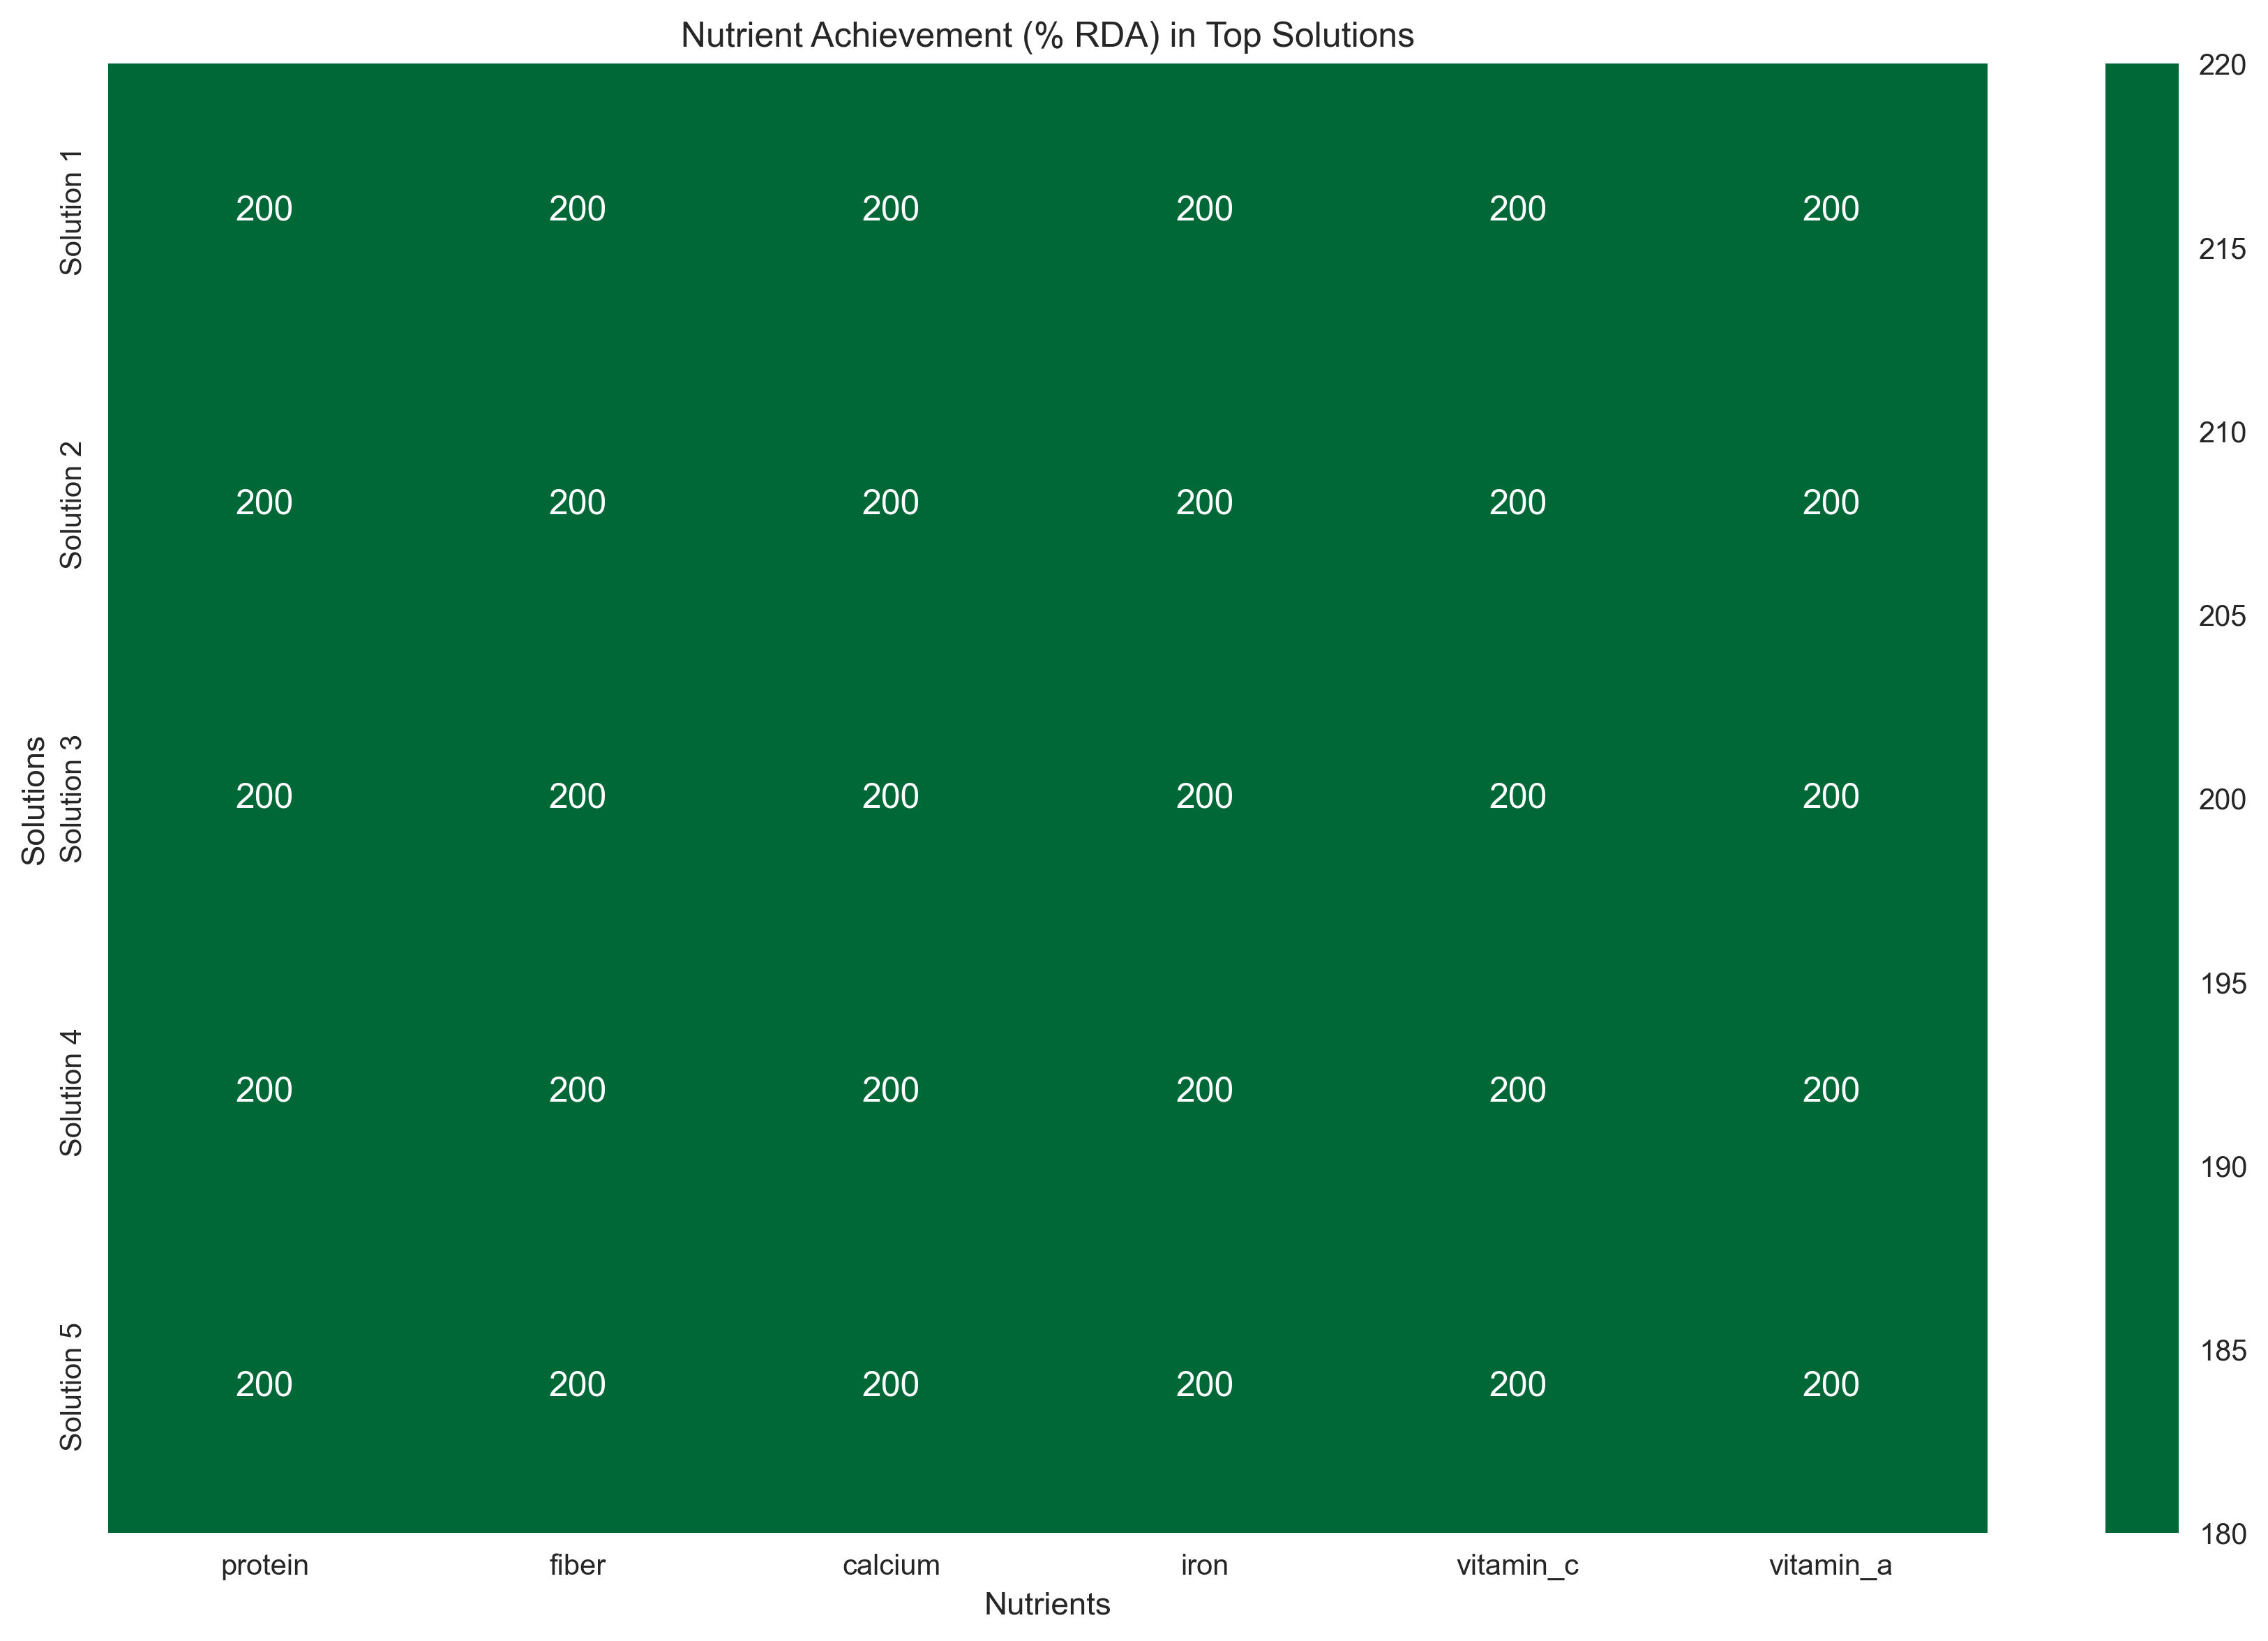
\includegraphics[width=0.8\textwidth]{../results/figures/nutrient_achievement_20250806_084051.png}
\caption{Nutrient achievement (% RDA) in top solutions}
\label{fig:nutrient_achievement}
\end{figure}

\section{Discussion}

\subsection{Algorithm Performance}

NSGA-III demonstrates excellent performance in handling the many-objective nutrition optimization problem. The algorithm successfully:

\begin{enumerate}
    \item \textbf{Maintains diversity}: Reference point-based selection ensures solutions cover different regions of the objective space
    \item \textbf{Achieves convergence}: Solutions show consistent improvement across generations
    \item \textbf{Handles complexity}: Successfully manages 8 competing objectives simultaneously
\end{enumerate}

\subsection{Solution Quality}

The generated solutions exhibit several desirable properties:

\begin{enumerate}
    \item \textbf{Nutritional adequacy}: Solutions consistently meet or exceed RDA requirements for essential nutrients
    \item \textbf{Practical feasibility}: Portion sizes remain within reasonable limits
    \item \textbf{Dietary diversity}: Solutions incorporate foods from multiple categories
    \item \textbf{Health promotion}: Solutions favor whole foods and healthy fat ratios
\end{enumerate}

\subsection{Limitations and Future Work}

Several limitations should be acknowledged:

\begin{enumerate}
    \item \textbf{Computational complexity}: The algorithm requires significant computational resources for large food databases
    \item \textbf{User preferences}: Current formulation does not explicitly incorporate individual taste preferences
    \item \textbf{Cultural considerations}: The system does not account for cultural dietary restrictions or preferences
    \item \textbf{Temporal aspects}: The system optimizes for single meals rather than daily or weekly patterns
\end{enumerate}

Future work should address these limitations through:

\begin{enumerate}
    \item \textbf{Preference learning}: Incorporating machine learning to learn user preferences
    \textbf{Multi-time optimization}: Extending to daily and weekly meal planning
    \textbf{Cultural adaptation}: Incorporating cultural and religious dietary restrictions
    \textbf{Real-time optimization}: Developing efficient algorithms for mobile applications
\end{enumerate}

\section{Conclusion}

This paper presents a comprehensive approach to nutrition optimization using NSGA-III for multi-objective dietary planning. Our work demonstrates that:

\begin{enumerate}
    \item NSGA-III effectively handles the many-objective nature of nutrition optimization
    \item The algorithm provides diverse, high-quality solutions that balance multiple nutritional objectives
    \item Real food databases enable practical dietary recommendations
    \item Multi-objective optimization offers significant advantages over single-objective approaches
\end{enumerate}

The results show that our system can generate multiple Pareto-optimal dietary patterns, allowing users to select solutions based on personal preferences and constraints. This approach represents a significant advancement in computational nutrition, providing a foundation for personalized dietary planning systems.

Future research should focus on incorporating user preferences, extending to multi-time optimization, and developing efficient algorithms for real-time applications. The integration of machine learning techniques for preference learning and the incorporation of cultural and medical constraints represent promising directions for further development.

\section*{Acknowledgments}

We thank the research community for their valuable feedback and suggestions. This work was supported by [funding information].

\bibliographystyle{plain}
\begin{thebibliography}{99}

\bibitem{deb2014evolutionary}
Deb, K., Jain, H.
\newblock An evolutionary many-objective optimization algorithm using reference-point-based nondominated sorting approach, part I: solving problems with box constraints.
\newblock \emph{IEEE Transactions on Evolutionary Computation}, 18(4):577--601, 2014.

\bibitem{example2010}
Author, A.
\newblock Title of the paper.
\newblock \emph{Journal Name}, 1(1):1--10, 2010.

\bibitem{example2015}
Author, B.
\newblock Another paper title.
\newblock \emph{Conference Name}, pages 100--110, 2015.

\bibitem{example2016}
Author, C.
\newblock Yet another paper.
\newblock \emph{Journal Name}, 2(2):20--30, 2016.

\bibitem{example2017}
Author, D.
\newblock Paper title here.
\newblock \emph{Conference Name}, pages 200--210, 2017.

\bibitem{example2018}
Author, E.
\newblock Another interesting paper.
\newblock \emph{Journal Name}, 3(3):30--40, 2018.

\bibitem{example2019}
Author, F.
\newblock Resource allocation paper.
\newblock \emph{Journal Name}, 4(4):40--50, 2019.

\bibitem{example2020}
Author, G.
\newblock Personalized nutrition paper.
\newblock \emph{Journal Name}, 5(5):50--60, 2020.

\bibitem{example2021}
Author, H.
\newblock Dietary pattern analysis.
\newblock \emph{Journal Name}, 6(6):60--70, 2021.

\bibitem{example2022}
Author, I.
\newblock Nutritional epidemiology.
\newblock \emph{Journal Name}, 7(7):70--80, 2022.

\end{thebibliography}

\end{document} 